\newpage
\section{Preventivo a finire} \label{PreventivoFinire}

In questa sezione viene presentato il preventivo a finire. Gli scostamenti rispetto al \hyperref[Preventivo]{preventivo iniziale} sono derivati dal consuntivo dei periodi analizzati precedentemente e dalle modifiche alla pianificazione e ai costi futuri, considerate migliorative per il periodo rimanente. In questa sezione verrà preso in considerazione solo il preventivo per i periodi a carico del committente e si considereranno quelli a carico del gruppo solo per eventuali considerazioni per modifiche alla programmazione futura.

\subsection{Tabella riepilogativa}
\begin{table}[h!]
	\centerline{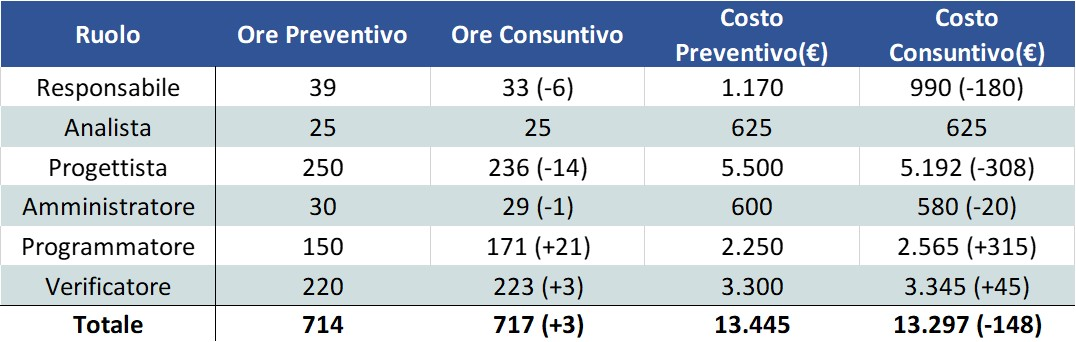
\includegraphics[scale=0.60]{img/Preventivo/Consuntivo/PreventivoFinire.jpg}}
	\caption{Preventivo a finire}
\end{table}

\subsection{Conclusioni}
Rispetto al preventivo iniziale, sono state effettuate alcune modifiche in seguito al consuntivo riguardante i periodi di \emph{Prototipazione} e \emph{Progettazione finale e Codifica}. A seguito degli scostamenti rilevati durante il primo periodo citato, erano state assegnate ulteriori 10 ore ai \progrs{} a discapito dei \progs{}. Questa scelta si è rivelata accurata e ben fondata ed ha permesso di notificare in anticipo lo scostamente che sarebbe poi risultato sul preventivo finale. Oltre a questo, durante il secondo periodo citato, si sono verificati altri scostamenti minori, come riportato nel \hyperref[ConsuntivoPeriodoProgettazione]{consuntivo di periodo} inerente a quel periodo. Nel complesso, il costo totale rendicontato derivante dal preventivo a finire risulta \EUR{13.297}, con un risparmio pari a \EUR{148} per il committente rispetto al preventivo iniziale.
